% COMS 6998, Fall 2026 -- P2: Prototype & Pilot Results
% Official course P2 template; supplied IEEEtran.cls and formatting retained.
% Source content: reviewed docs/MILESTONE2.md and saved pilot evidence.
\documentclass[conference,10pt,letterpaper]{IEEEtran}
\usepackage[T1]{fontenc}
\usepackage{cite}
\usepackage{graphicx}
\usepackage{booktabs}
\usepackage{tabularx}
\usepackage{flushend}
\usepackage[hyphens]{url}
\usepackage[hidelinks]{hyperref}

\newcommand{\field}[1]{\textit{[#1]}}

\title{B5: E-Graph-Augmented Tool-in-the-Loop RTL Verification}
\author{\IEEEauthorblockN{Chiyu Chen (cc5583), Mingyuan Zheng (mz3143), Yiwen Chen (yc4653)}
\IEEEauthorblockA{COMS 6998: AI-Native Computing $\mid$ Fall 2026\\
P2: Prototype \& Pilot Results $\mid$ Due November 9, 2026, 11:59 PM ET}}

\begin{document}
\maketitle
\thispagestyle{plain}
\pagestyle{plain}

\section{Project Goal and Updates}
Our project asks whether E-graph semantic feedback helps an LLM verify RTL more
effectively and efficiently than raw execution feedback. The proposal compares
text-only (A), raw-coverage (B), and E-graph-enhanced (C) stimulus generation.
That track already has exploratory coverage pilots. Our separately authorized
\emph{test2} extension fixes the stimuli and asks the LLM to generate passive
SystemVerilog monitors. It measures valid fault detection, false alarms, and
cost. This separates the quality of a generated checker from the model's ability
to choose inputs and provides a complementary test of the proposal's central
semantic-feedback hypothesis.

This endpoint change is explicit: changing a monitor under fixed stimuli does
not improve DUT coverage. Raw source coverage supplies feedback and workload
context; monitor quality is the outcome. We do not claim an official CVDP or
Pass@1 evaluation. Current results are descriptive pilots, and a negative C/B
comparison remains useful evidence. Our next priority is a bounded comparison
on a different protocol IP rather than extending a general verification-tool
qualification framework.

\section{Method Overview}
The implemented loop freezes the DUT, specification, inputs, reference, model
settings, and resource caps. Python orchestrates GPT candidate generation,
compilation and public development feedback, per-round snapshots, final release,
hidden grading, replay, and reporting. A Rust \texttt{egg} pipeline forms
restricted equivalence groups. Typed complete guards and independent Z3 checks
retain widths, signedness, activation conditions, and clock/reset context.
These checks establish limited two-state combinational relations, not general
sequential or four-state equivalence. Equivalent guards retain their distinct
original source counters.

A Claude-authored specification reference remains independent of GPT's candidate
monitors. Candidates cannot grade themselves. Public prompts exclude the
reference implementation, hidden faults, final evaluation traces, and solver
witnesses. B receives the specification, permitted RTL, fixed development
observations, raw counters, and its own development feedback. C receives the same
information plus validated E-graph relations. Within each arm, sessions are
independent; all rounds are frozen before hidden scoring. The final candidate
is selected by the registered validity/compilation rule, not its hidden score.

The controller study uses \texttt{gpt-6.1-sol} with low reasoning, three sessions
per arm and six rounds per session, for 36 generation calls. Each call has the
same 64k-input/8,192-output token caps. Equal caps do not imply equal spending.
A final-post \texttt{trace\_done} marker exposes the finite evaluation boundary
to a passive monitor without adding a DUT input or clock edge.

Scoring first checks finite correct-DUT controls. Fault credit requires an
independent reference-confirmed observable violation and an eligible candidate
alarm; earlier alarms cannot earn credit. Invalid candidates, unknowns,
unobservable fault types, and failures remain in the evidence. Repeated alarms
and two simulators do not create additional defect types. API tokens,
compilation, physical DUT simulation/cycles, monitor replay, and wall time are
recorded separately. Without a token-matched placebo, B/C compares the complete
feedback package rather than isolating semantic content from extra context.

\section{Prototype and Pilot Results}
\textbf{What runs end to end.} The saved multi-cycle request/response controller
study includes fixed physical observations, monitor generation, compilation and
development feedback, candidate freeze, hidden grading, saved-response replay,
and a result report. Concrete inputs are
\path{test2/configs/controller_done_study_v1.json} and
\path{test2/tasks/axis_length_done_v1/} input/evaluation freezes. The generation
entry is \path{test2/scripts/controller_done_generate_v2.py}; the postprocessing
entry is \path{test2/scripts/controller_done_live_post_v2.py}. The live run's
\texttt{release.json} and \texttt{final-candidates.json} bind its candidates.
The live and saved-response replay paths have separately saved scores.

The original final audit adapter failed on a catalog-field mismatch. That
failure is preserved. A new read-only adapter recovered the audit from already
saved evidence without rerunning model generation or physical/formal
experiments. Thus the prototype has executed end to end with documented recovery;
we do not present it as a fresh, clean single-command run. Historical commands,
exits, and recovery are retained in the postprocessing progress files.

\begin{figure*}[t]
\centering
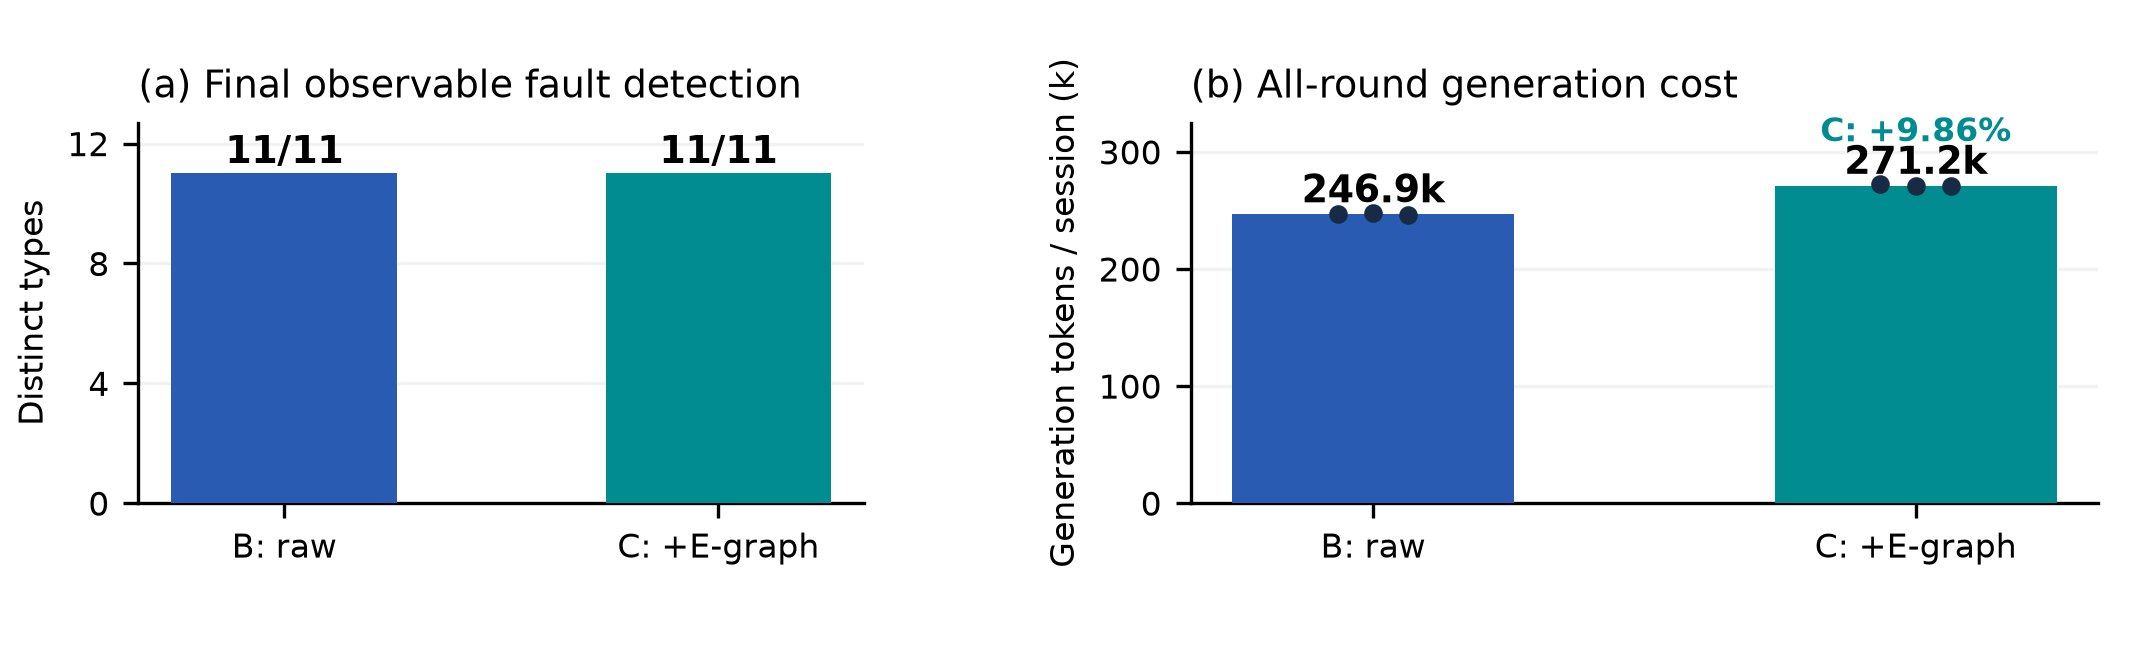
\includegraphics[width=\textwidth]{images/pilot-bc.png}
\caption{Saved controller fixed-stimulus pilot: three independent sessions per
arm, six rounds each (36 generation calls). All six final monitors detect 11/11
confirmed observable types; the raw denominator remains 12, including N10 whose
observability was not confirmed. Right: mean actual generation input+output
tokens over all rounds; dots are session totals. B totals 740,643 tokens and
C 813,649, a 9.8571\% C increase. Cache/reasoning subcounts are included, not added
again. This figure excludes compilation/simulation/wall costs and is not an
invoice, significance test, or general correctness claim.}
\label{fig:pilot}
\end{figure*}

\textbf{Observed comparison.} All six final selected monitors pass 18 finite
correct-control cases each and detect 11/11 confirmed observable injected fault
types (Fig.~\ref{fig:pilot}). The original denominator is 12 types/144 fault pairs;
N10 is retained as not confirmed observable. B uses 740,643 generation tokens
across its 18 rounds, versus 813,649 for C: C uses 9.8571\% more, with no extra final
fixed-trace kills. Per-session means are 246,881 and 271,216.33 tokens. The score
is a finite, unattributed case/type union, not a proof that each monitor slot
checks a particular semantic category.

Unknowns are not converted to passes: 38 reference-unknown pairs remain per
candidate, and one B candidate has 40 total unresolved pairs after its candidate
unknowns are included. Earlier invalid rounds and their generation costs remain.
The separate formal schedule retains 75 PASS, 104 FAIL, and 361 TIMEOUT statuses over 540
jobs, including 74 unreproduced/unresolved BMC witnesses. Native failures are not
pooled as confirmed detected faults, and no 128-cycle completion proof follows.

The exact numeric source is
\path{test2/results/controller-done-live-acceptance-v3/audit.json}; the scoped
report is \path{test2/results/controller-done-live-report-v4/report.md}.
This P2 figure was rendered from that saved cohort; no research experiment was
rerun to prepare this report. The observed endpoint is saturated, so the result
supports no additional final C benefit on this workload, not a universal claim
that E-graph feedback cannot help verification.

\section{Next Steps}
\textbf{Main risk.} A small, saturated fault set offers little room to distinguish
B from C, while longer C prompts confound semantic value with context cost.
One inspected IP and three sessions per arm do not establish cross-IP
performance or statistical significance. We will preserve this tie and its
costs rather than change labels or targets to obtain a positive result.

Toward Milestone~3 on Nov~23, our next bounded pilot is OpenTitan I2C READB with
one ACKing target. Existing assets include original RTL/specification, a fixed
driver, calibration observations, a finite Claude reference, and validated guard
relations. A one-page task card, a 32-field public observation mapping, role
allowlists, and a reference-scope review prompt are prepared. The new test2 SV
adapter, disjoint hidden inputs, and physically observable DUT mutants are
\emph{not implemented or tested}. Old trace-corruption controls are not RTL
defects and will not substitute for physical mutant qualification.

Before candidate calls, we will check only the adopted input/reset/first-sample
and pre/post path, positive/negative/unknown controls, independent reference
scope, fixed data, and prompt isolation. A fresh independent Claude review must
confirm the existing finite oracle's permitted scope; any required oracle
change needs a separate Claude author and fresh reviewer. GPT will not silently
repair it. Pending/invalid traces and the existing stretch, liveness, extra-STOP,
and 256-byte completion limits remain. Generic formal-tool qualification is
paused with its failures and costs preserved; it is not an unlimited prerequisite
for this separate finite simulation study.

The proposed small I2C comparison has two independent sessions per arm and three
rounds, with identical model/caps, selection, fixed stimuli, and hidden grading.
Actual settings, rates, and service budget still require a concrete online
decision. No new I2C live results or paid calls are claimed here.

\textbf{Midterm feedback response pending.} Actual instructor/TA technical
feedback has not been provided or located in the bounded local search. We will
record the original comment, resulting change, evidence, and limitation when it
is available. The user's prioritization of cross-IP work and internal reviews
are not substituted for classroom feedback.

\end{document}
